%
% OPUS Manual
%

% Latex 2e

\pdfcompresslevel=9
\pdfoutput=1

% Try 12 point
\documentclass[12 pt]{book}
%
% Pick one of the following font packages (if you don't like CM)
%
%\usepackage{pslatex}
\usepackage{times}
%\usepackage{palatino}
%\usepackage{newcent}
%
%
\usepackage{hyperref}
\usepackage{makeidx}
\usepackage{fancyhdr}
\usepackage[pdftex]{graphicx}
%\usepackage{amsfonts}
\usepackage{url}
\usepackage{color}
\usepackage{listings}
\usepackage{layout}
\usepackage[margin=3cm,innermargin=1.5cm,outermargin=1cm,includemp=true,marginparsep=1 cm, marginparwidth=2.5 cm, paperwidth=190 mm,paperheight=260 mm]{geometry}
\usepackage{ifthen}
%
% Define some dingbats
%
\usepackage{pifont}

%
% Change the default bullet
%
\renewcommand{\labelitemi}{%
        \raisebox{-.25ex}{\ding{43}}}

%
% Does it all have to be Arial now? <sigh>
%
\renewcommand{\familydefault}{\sfdefault}

\DeclareGraphicsExtensions{.pdf,.png,.mps}

\pdfinfo{
  /Title (OPUS Manual)
  /Author (Dr Colin Turner)
  /Producer (PDFLaTeX)
}

\makeindex

\begin{document}

% New commands, and notation
%
% Preamble for all documents
%
% Colin Turner
%

% Latex 2e

\newcommand{\UniversityName}{the University of Ulster}
\newcommand{\ShortUniversityName}{Ulster}
\newcommand{\OpusUrl}{http://opus.ulster.ac.uk}
\newcommand{\DevelopmentUrl}{http://foss.ulster.ac.uk/projects/opus/}
\newcommand{\ContactEmail}{opus@foss.ulster.ac.uk}

% Headings
%
% Headings for notes
%
% Colin Turner
%

% Latex 2e

% Headings



%
% New fancyhdr version
%
\pagestyle{fancy}
\addtolength{\headwidth}{\marginparsep}
\addtolength{\headwidth}{\marginparwidth}
\renewcommand{\chaptermark}[1]{\markboth{#1}{}}
\renewcommand{\sectionmark}[1]{\markright{\thesection\ #1}}
\fancyhf{}
\renewcommand{\headrulewidth}{0pt} % get rid of the line
\fancyhead[LE,RO]{\colorbox{cyan}{\color{white}\thepage\normalcolor}}
\fancyhead[LO]{\colorbox{cyan}{\color{white}\rightmark\normalcolor}}
\fancyhead[RE]{\colorbox{cyan}{\color{white}\leftmark\normalcolor}}
\fancypagestyle{plain}{%
\fancyhead{} % get rid of headers
\renewcommand{\headrulewidth}{0pt} % and the line
}

%
% Now some LaTeX magic from
% http://research.cmis.csiro.au/gjw/tex/docs/fancyhdr.pdf
% to make extra pages blank
%


\makeatletter
\def\cleardoublepage{\clearpage\if@twoside \ifodd\c@page\else
\hbox{}
\vspace*{\fill}
%\begin{center}
%This page intentionally contains only this sentence.
%\end{center}
\vspace{\fill}
\thispagestyle{empty}
\newpage
\if@twocolumn\hbox{}\newpage\fi\fi\fi}
\makeatother


% Listings package
\lstset{
  language=PHP,
  alsolanguage=HTML,
  basicstyle=\ttfamily,
  flexiblecolumns=true,
  lineskip=-2pt,
  commentstyle=\color{blue},
  morecomment=[s][\color{red}]{/**}{*/},
%  frame=l,
  numbers=left,
  numberstyle=\tiny,
  stepnumber=5,
  numbersep=5pt,
  backgroundcolor=\color[rgb]{0.95, 0.95, 0.95}
}


% New environments

\newcommand{\pdstext}[1]{\color{magenta}{\sffamily\bfseries #1}\normalcolor}
\newcommand{\opusurl}{http://opus.ulster.ac.uk}
\newcommand{\opustext}[1]{\color{magenta}{\sffamily\bfseries #1}\normalcolor} 
\newcommand{\opusstudentmenu}[1]{\color{blue}{\ttfamily \bfseries #1}\normalcolor} 
\newcommand{\opusacademicmenu}[1]{\color{red}{\ttfamily \bfseries #1}\normalcolor} 
\newcommand{\pdsiconcd}{\marginpar{
\includegraphics[scale=1.0]{png/icon_cd.png}}}
\newcommand{\pdsiconsa}{\marginpar{
\includegraphics[scale=1.0]{png/icon_sa.png}}}
\newcommand{\pdsiconmc}{\marginpar{
\includegraphics[scale=1.0]{png/icon_mc.png}}}
\newcommand{\pdsicons}{\marginpar{
\includegraphics[scale=1.0]{png/icon_s.png}}}
\newcommand{\pdsiconpt}{\marginpar{
\includegraphics[scale=1.0]{png/icon_pt.png}}}
\newcommand{\pdsbookletref}[1]
{\marginpar
  {\makebox[0 pt][l]
    {
\includegraphics[scale=1.0]{png/icon_book.png}
  }
  \parbox{2 cm}{{\sffamily \bfseries \tiny #1}}}}

\newcommand{\pdstip}[1]{{\bfseries TIP!} \emph{#1}}
\newcommand{\opustip}[1]{{\bfseries TIP!} \emph{#1}}

%
% Page Dimensions, required to be custom for this job
%
\setlength{\paperheight}{260 mm}
\setlength{\paperwidth}{190 mm}
\setlength{\pdfpageheight}{\paperheight}
\setlength{\pdfpagewidth}{\paperwidth}


\title{OPUS Manual}

\author{Dr Colin Turner\\\url{c.turner@ulster.ac.uk}}

\date{July, 2008}

%%% ----------------------------------------------------------------------

\pagenumbering{roman}
\maketitle

\pagestyle{fancy}

\tableofcontents
\markboth{Contents}{Contents}

%\listoftables

%\listoffigures

%
% Introduction, unnumbered chapter
%

\setlength{\parindent}{0 cm}
\setlength{\parskip}{0.2 cm}

\chapter*{Introduction\markboth{Introduction}{}}
Welcome to the OPUS manual. As you will see this is really a work very much in progress. Please note that the most up-to-date version will always be
found at the development site for OPUS at \url{http://foss.ulster.ac.uk/projects/opus}, currently only in source repository, but hopefully we will enable
automatic builds of the documentation in the near future.

%\newpage
%\pagecolor{red}
%\pagecolor{white}
%\newpage

\chapter{How to use this workbook}
\pagenumbering{arabic}

You 
might choose to read this workbook from cover to cover,
or to dip into it as required. The following conventions
have been 
used to help you get the most of this book whatever way you choose to use it. 

\section{Signposts}
\index{Signposts}

At various points in the workbook, signposts are used in
the margins to indicate that a section is of specific
interest to a particular role you may have.

\parbox{2 cm}{
\includegraphics{png/icon_cd.png}}
\parbox{9 cm}{Course Directors ({\bfseries CD}) have many varied responsibilities,
including often acting as an Adviser of Studies.}
\index{Course Director}
\medskip

\parbox{2 cm}{
\includegraphics{png/icon_sa.png}}
\parbox{9 cm}{Studies Advisers ({\bfseries SA}). The PDSystem has a great deal of
dedicated support for the studies advice process.}
\index{adviser of study}
\index{studies adviser|see{adviser of study}}
\medskip

\parbox{2 cm}{
\includegraphics{png/icon_mc.png}}
\parbox{9 cm}{Module Coordinators ({\bfseries MC}). Many
of the facilities useful to Course Directors are also
useful to Module Coordinators.}
\index{Module Coordinators}
\medskip

\parbox{2 cm}{
\includegraphics{png/icon_s.png}}
\parbox{9 cm}{Supervisors ({\bfseries S}). For the purposes
of this workbook, supervisors are taken to include those
responsible for undergraduate projects, right up to PhD
supervision.}
\index{Supervising}
\medskip

\parbox{2 cm}{
\includegraphics{png/icon_pt.png}}
\parbox{9 cm}{Placement Tutors ({\bfseries 
PT}). The PDSystem provides many possibilities for
monitoring and assessing placements, and integrates into
OPUS. OPUS is another University of Ulster on-line system
which deals comprehensively with the whole
placement process: it aids in the tasks of finding students
a placement; recording their placement information,
assessing their placement and more. More details can
be found at \url{http://opus.ulster.ac.uk}.}
\index{placement!tutors}

\section{Typographical Conventions}
\index{typographical conventions}

Text which appears on OPUS screens will be
presented \opustext{like this}.

Where specific menu selections on OPUS are detailed they will
be shown as follows: 
\begin{itemize}
\item \opusstudentmenu{Section -> Subsection} when the student strand is discussed; and
\item \opusacademicmenu{Section -> Subsection} when the staff strand is being discussed.
\end{itemize}

\opustip{Sometimes an important tip will appear like this}.

\part{Administration Guide}

\chapter{Installation}
\index{installation}

We look at the various requirements of OPUS here and how to install it.

\section{Requirements}
\index{installation!requirements}

OPUS can be run on top of  any system that supports PHP%
\footnote{A popular web scripting language (\url{http://www.php.net})} and MySQL.%
\footnote{A relational database engine (\url{http://www.mysql.com})}

At the time of writing, specific requirements are
\begin{itemize}
  \item PHP version 5.1 or higher;
  \item MySQL version 4 or higher;
  \item Smarty\footnote{A templating engine (\url{http://smarty.php.net})} version 1.3 or higher;
  \item Pear;%
    \footnote{Extensions to PHP, found at \url{http://pear.php.net}. Pear is required for logging support.}
  \item Perl version 5 or higher.\footnote{A powerful scripting language, required for some offline maintainence, available from \url{http://www.perl.com}.}
\end{itemize}

Some (optional) functionality uses Unix command line tools that will almost certainly be present on
any modern Unix or Linux system. If you are using Windows, you can obtain free versions of such
software for that platform.\footnote{See \url{http://unxutils.sourceforge.net/} for example.}

\section{Operating Systems}
\index{operating systems}
\index{Debian GNU/Linux}

It should be straight forward to install OPUS on most variants of Unix, or Linux and, with perhaps some more work, Microsoft Windows.

\subsection{GNU/Linux}

Various distributions of GNU/Linux, or simply Linux, as they are often called, are well suited to running OPUS. Almost all modern versions
package all or most of the requirements listed above.

The absolutely simplest way is to install OPUS on a server running Debian GNU/Linux 4.0 (Etch) or above%
\footnote{Available for many architectures from \url{http://www.debian.org}.}%
since OPUS is specifically \emph{packaged} for Debian.

Indeed, using the Debian packages will allow you to greatly circumvent many of the other issues in this, and the following chapter, since
much of the installation and packaging will be handled automatically.

To ensure automatic installation and upgrades, add the following line to your configuration for \lstinline!apt! usually found in
\lstinline!/etc/apt/sources.list!.

\begin{lstlisting}
deb http://foss.ulster.ac.uk/debian stable main
\end{lstlisting}

\subsection{Unix}
\index{Unix}

As Unix and GNU/Linux are very closely related, most versions of Unix will also run OPUS with ease. Again, most modern Unix versions
provide packaged versions of the requirements, or most of them.

\subsection{Microsoft Windows}
\index{Windows (Microsoft)}

At this time Windows cannot be recommended for running OPUS since
\begin{itemize}
  \item in \emph{very} rare places OPUS calls standard unix style utilities; in particular it uses \texttt{grep} and \texttt{tail} in its log
    file viewer. These tools can be obtained for the Windows platform however;
  \item OPUS runs scheduled jobs using \texttt{cron} to perform regular maintainence, you will need to trigger these with the various
    scheduling tools available on the specific version of Windows you are running (see \texttt{at}) for example;
  \item OPUS has been designed and run on Linux and Solaris, at present the various installation scripts and snippets we have produced
    are aimed at such platforms. However, please \emph{do} feel free to send patches with better Windows support.
\end{itemize}

This is \emph{not} to say that OPUS cannot be run on Windows, and if you have expertise with Windows you will have no problems overcoming these
hurdles by yourself.

\section{Manual Installation}

If you plan to install OPUS manually, here is some guidance on the important directories you need to manage.

\begin{description}
  \item[include] contains vital files that the ``main'' scripts of OPUS will use. This should \emph{not} be installed in the web server document root, since
  it also contains sensitive configuration. However, the web server will need read access to these files.
  \item[html] contains the ``main'' scripts and content that OPUS provides. This will need to be in the web server tree.
  \item[templates] contains Smarty templates for output, like include, it should be outside the document root, but accessible to the web server.
  \item[cron] contains PHP scripts that perform automatic maintainence. 
  \item[docs] contains files to produce this manual, not required on a production server.
  \item[etc] contains an example Apache configuration file, suitable for Debian.
  \item[sql\_patch] contains SQL files for importing the intial schema and data into MySQL.
\end{description}

In addition, you should create two more directories, probably in \lstinline!/var/lib/opus/! or an
equivalent directory on your operating system. 

\begin{description}
  \item[templates\_c] used by smarty to compile templates, note it \emph{must} be writable by the web server process.
  \item[templates\_cache] used by smarty for various caching, again, must be writable by the web server.
\end{description}

To set the correct permissions you could use commands like:

\begin{lstlisting}{language=bash}
chown root:www-data templates_*
chmod 770 templates_*
\end{lstlisting}

where \lstinline!www-data! is the username for the web server process.

One easy way to deal with this is to copy the whole set into a location \emph{not} under the web server tree, and configuring the web server to have
acess to the html directory only. For Apache, this is more or less done with the file in the etc directory. You will note it also changes the PHP include
path to use the include path, as well as a Smarty path. You might need to change paths accordingly.

\subsection{Configuring your Web Server}

You will now need to ensure that your web server can ``see'' the directories it will need access to. There are several ways to achieve this.

\subsubsection{Directly copy under the web server root}

Perhaps the simplest approach is to copy the \lstinline!html! directory under the web server root. It is \emph{not} recommended that any other
paths are copied in this way for security reasons. This is probably simple, but tedious in the long run since it will make upgrades more difficult.

\subsubsection{Use a symbolic link}

If you are using an operating system that supports symbolic links, you could link the \lstinline!html! directory to a path under the main web server
document root.

\subsubsection{Using a configuration file}
\index{Apache}

Probably the most flexible and elegant way it to use a configuration file. If you are using Apache 2 you will find a suitable configuration file in the
\lstinline!etc! directory of the OPUS package. Simply copy it to your appropriate configuration directory for apache (probably something like
\lstinline!/etc/apache2/conf.d/! and edit to requirements. Then restart the web server.

\opustip{You will need to ensure that PHP includes the appropriate directories from OPUS and Smarty in its local include path. Although you can do this
by editing the global \lstinline!php.ini! file, it is easier to do this as a local override. The configuration file does this for you. If you use an alternative
method you will almost certainly need to include a file (like \lstinline!.htaccess! for Apache) that overrides this path.
\emph{make sure your \lstinline!include_path! does not include the current directory (.)}, or if
it does, ensure that this is included last on the include paths.}

\subsection{Database Creation}
\index{MySQL}

You should now create a new database. Using your mysql client or otherwise. To use the client, launch it from the
command line like so. If you have (correctly) configured a password for the root user add \lstinline! -p ! to this command.
\begin{lstlisting}[language=bash]
mysql -u root
\end{lstlisting}
or using a password as required. At the client prompt, create a new database
\begin{lstlisting}[language=SQL]
create database opus;
grant all on opus.* to opus_user@localhost
  identified by 'database_password';
\end{lstlisting}

You will need to modify this if the database is on a remote host accordingly. At this point
you can import the schema files from the sql\_patch directory.
\begin{lstlisting}[language=SQL]
source sql_patch/schema.sql
source sql_patch/data.sql
\end{lstlisting}

\subsection{Logging}

OPUS uses substantial logging throughout, and maintains several log files. You should ensure that you have a directory created to which
the web server has write access. See the discussion for the templates directory above. This can be anywhere, such as \lstinline!/var/log/opus/!.

\chapter{Administrators \& Policies}
\index{security}
\index{access}
\index{administrators}
\index{policies}

This chapter is required reading for the top level administrators of OPUS, it
is of less interest to other administrators who should find that things are
already correctly configured for them.

You should login with the newly installed ``Super-Admin'' user account. This
user has no security restrictions imposed on it, and it is unwise to use it
for day to day purposes. Therefore you will want to make one or more ``normal''
administrator accounts.

\opustip{The initial login credentials will be \lstinline!admin! and 
\lstinline!password! so it is obviously absolutely essential that you change 
the password as soon as possible, and certainly before importing other data.}

Normal administrator accounts are bound by \emph{security policies}. These
define the range of actions that may be undertaken by the user. In addition, 
each administrator may be limited in scope so that they may exercise their
powers on an institutional level, or at faculty, school or individual
programme, or even a combination of the above.

\section{Policies}
\ref{Policies}
\index{policies}

You should begin by considering your security policies. By clicking on
\opusacademicmenu{Advanced -> Policies} you will be able to view and manipulate
policies. OPUS already comes configured with a number of policies, that you may
wish to add to, or adjust.

More or less, \emph{Placement Coordinators} operate at a high level
institutionally, should be better trained with OPUS and well versed in your
policies for adding companies. Out of the box, they can add companies and other
details that lesser users can only edit.

By contrast, \emph{Placement Tutors} usually have responsibility for a few
programmes. They have less power, but remember, you can \emph{help} staff by
restricting their access so they can't make foolish errors.

The \emph{Viewer} policy is intended for staff who need read only access to
data but should never make changes.

The \emph{Priority} attached to a policy simply dictates a kind of distance
from the students. The lower the priority, the closer a policy holder is to
the students, and so it is assumed they will be able to help more fully deal
with queries about individual students.

Clicking on \emph{Permissions} shows the complete list of permissions for a
policy. Only super-admin users can make changes, but other admin users can
see the details of their own policy.

\subsection{Adding a Policy}

Choose a name that reflects your policy and submit it. You are now able to
edit the permissions for that policy. One of the first options is a priority
for use in the help directory (see~\ref{HelpDirectory}).

The lower the priority, the 
``closer'' this group is to the students, and therefore the
higher up such users will appear in the dynamic help directory.

You may now check and uncheck boxes as you wish to allocate permissions. 
In general, the recommendations are that
\begin{itemize}
  \item Very few, if any, users should be able to delete items - it damages
    the ability to use OPUS as an audit tool.
  \item Few users should be able to create items - these users should be well
    trained and able to act coherently as a group.
  \item Give day to day administrators more abilities to edit than create or delete.
  \item It is possible to create policies that can ``look but not touch'' for those
    users who only need read access to data.
\end{itemize}

In general a hierarchy of at least a couple of policies is recommended, to put
more experienced users in the higher bracket.

\section{Administrator Users}

Now you have created suitable policies, you are ready to create administrator
users and allocate them to policies. A policy provides a ceiling on the powers
of a user - it is possible to curtail them further as needed (see~\ref{}).

Clicking on the \opusacademicmenu{Directories -> Administrators} menu item will 
allow you to list and create new administrator users. As is often the case 
within OPUS, you should start by searching for the user to ensure they are not
already present before the \emph{add} button will present itself.

\subsection{Creating Administrators}

Adding an administrator can only be performed by a super-admin user, and quite
a bit of information is required. Add all the required fields, and note in
particular these others. When a user is created, they will be emailled their
initial username and password.

\subsubsection{Policy}

If no policy is defined, this user will not be able to do anything. Select an
appropriate policy having read the details above.

\subsubsection{Institutional Admin}

Sometimes a member of staff will need rights over the whole institution, but
not at a super-admin level. Rather than add them to each faculty, you can
choose to make them an institutional admin, in which case they will see all
programmes of study, and potentially all students. There should be 
\emph{very few} such users.

\subsubsection{Help Directory}

This dictates whether a user will appear in the dynamic help directory. You
should add members of staff who should be contacted by students and outside
companies here. Members of staff on holiday should be temporarily removed.

\subsubsection{Reg Number}

If the staff number is defined, it may be possible to login using a ``standard''
single sign-on method, depending on how your OPUS is configured. It is also
required for automatic saving of preferences.

\subsection{Editing Admin Details}

If you are a normal administrator you will only have permission to edit your own
account, and will not be able to edit other accounts.


\subsection{Promotion}
\index{root users}

You can (if you are a super-admin user), promote another admin to super-admin
status. This should be done with \emph{great care}!

\subsection{Assigning Administrators to Academic Units}

While you will have some administrators who are appointed at an \emph{institutional}
level, that is they exercise their powers over all academic units in the institution,
it is more common that administrators act over a faculty, school, or programme.

Later, once you have defined your organisation within OPUS (see~\ref{Organisation}),
you will be able to assign administrators to these units.

\section{Super-Admin Users}

These users have a directory of their own, which allows them to be edited,
and demoted. Note you cannot directly create a super-admin user, you must 
create a normal admin user and promote them. This is not a bug.

You should generally keep \emph{very few} root accounts on your system.

\chapter{Initial Configuration}

After installation, it is usually necessary to copy the file
\lstinline!local.config.php.dist! to \lstinline!local.config.php! (in the 
\lstinline!include! directory) and customize its values.
\footnote{Debian installation will take care of this aspect, in Debian installs
you will find the local file in \lstinline!/etc/opus!.}

\section{Organisation Details}
\ref{Organisation}

OPUS will need to know something about the way in which your organisation is
set-up. Clicking on this menu item will take you to an option to configure the
faculties that will use OPUS.

\subsection{Faculties}

Create a new faculty by using the \opustext{add}
button. You will asked for a name, an optional web address, and an optional SRS
(Student Records System) code. If your system has a unique short identifier for
the faculty place it here.

Once a faculty is created, you can assign administrators that will have a role
over an entire faculty, or edit the schools within that faculty. Faculties can
be marked as \opustext{archive} which means they are no longer active (do not
delete records unless you have added them in error, old records should be
archived).

\subsection{Schools}

This operates in an identical way to the faculty list, create schools and if
desired, assign administrators to them. You can edit and move a school to
another faculty once created by changing the faculty in the drop down box.

\subsection{Programmes}

Finally we come to programmes of study. Again, you should specify the name, and
code for the programme, and also decide on the \emph{CV Group} if you want
different handling for this course.

It is also possible, from the programme list, to assign administrators to an
individual programme, if no-one already assigned at institutional level,
faculty level or school level will do. Furthermore, clicking on assessment
allows you to configure the assessmentgroup that a programme belongs to. This
can change over the years, so it is possible to declare the start and end years
for each association. Again, you should not delete older associations.

\section{CV Groups}

This section allows you to configure the way in which CVs should be handled.
You can create as many CV Groups as you wish, and each one can contain as many
programmes as you wish from a single unusual case, to all your programmes of
study.

OPUS already ships with a Default Group which all programmes belong to unless
you change them.

\subsection{Adding a CV Group}

To add a CV Group simply click the \emph{add} button on this screen. You should
use a simple, easily understood name for the group, and you can add a detailed
description of the rationale for this group if you choose.

Editing the Permissions allows you to select if all PDSystem templates should 
be allowed (assuming the PDSystem is available to you), and whether custom CVs
should be allowed.

\subsection{Editing a CV Group}

Once you have created a group, when it appears in the listing, there will be
an option to specify how \emph{templates} are handled. If you have a coupled
PDSystem this will produce an up-to-date list of templates offered by the
PDSystem, and you can choose whether each template is allowed by that group
for applications for placement, and, whether any such template based CV must 
be approved before use.

You can also select a default template which will be suggested to the student
when they make an application.

Remember, if you have selected to allow All PDSystem templates, this screen
will have no effect.

\subsection{Assigned Programmes to Groups}

Once your CV Group is created, you should edit the programmes you wish to move
into it, and simply change the CV Group to your new choice.

\section{Assessment Groups}

Assessment Groups allow you to decide how students will be assessed within
OPUS. Before this will be of any use, you must have configured some assessments
within the Advanced menu.

A Default Scheme already exists within OPUS which has no assessments added to
it. You should be cautious about changing groups, and read this section
carefully before hand.

\subsection{Adding an Assessment Group}

Adding an assessment group is as simple as clicking on the \emph{add} option
within this section. All that can be added is a name (which as usual should be
clear and distinctive) and some comments to describe the rationale of the
group.

\subsection{Changing the Regime for a Group}

Once a group has been created, clicking on \emph{regime} within its listing
will allow you to alter the assessments associated with it.

\pdstip{Generally, you should \emph{never} alter the regime for any group that
is in current use unless you absolutely know what you are doing. You may make
it impossible to retrieve marks already recorded for this group.}

\subsubsection{Adding Assessments}

Clicking on \emph{add} allows you to choose from the available assessments to
add to your regime. You can use a given assessment more than once if that is
appropriate.

You will see a pull down box of all the available assessments, and you should
add a unique description, within your regime to describe this instance,
together with a weighting (number between 0 and 1) that describes how much this
is worth, for example 0.3 represents $30\%$. You should also choose who will
perform the assessment.

Next comes the year, which is the year, relative to placement that the
assessment will take place. That is, for an assessment that takes place in the
year of placement, enter zero, for an assessment that takes place the previous
year, enter $-1$ and $1$ for the year after placement and so on. The
\emph{start} and \emph{end} dates should be specified in the MMDD form when
the assessment should be due, and completed. This is used to guage when 
assessments are late.

\subsubsection{Editing and Removing Assessments}

You can edit and remove assessments, but again, this can cause already submitted
marks to become inaccessible (not deleted, but essentially lost in the database),
so only certain users can perform these actions, and generally they are for the
design phase of assessment groups not currently used.

\subsection{Changing Regime for a Programme}

Assessment needs change, but generally you should create a brand new assessment
group if that happens, and record that the programme changed from one to 
another in a given year. This is the only was to guarantee access to old
marks in the old regime as well as new ones.

\section{Channels}
\label{Channels}

Channels are a relatively advanced topic, and on a relatively small OPUS
installation they may not be necessary at all. If however you have diverse
groups of students to deal with, read on.

A channel is a means to restrict the audience of some aspect of communication,
and so allows you to create a more local feel for a group of students in what
might otherwise be a very anonymous system. Various parts of OPUS, in particular
the resources and help systems can be customized by channels.

OPUS comes installed with a special \emph{Global} channel, to which all users
belong.

\subsection{Adding a Channel}

To add a channel, first list them by selecting the 
\opusacademicmenu{Advanced -> Channels} option. To add a channel very little
information is required, first of all a short name, which should be clear,
unique and distinctive; together with a short description of the channel
membership.

e.g. SSS - School of Sports Studies

\subsection{Editing Channel Associations}

Now we can edit the channel associations to determine who is included within
the channel. An \opustext{associations} action is shown in the channel list.

This will list the existing associations, and allow new associations to be
made. These essentially fall into five categories, and each assocition 
indicated a value of ``Enable'' or ``Disable'' together with an order. You
can move associations up and down the list and remove them. Currently you
cannot edit an association, simply remove it and add a new one.

This is quite a flexible system, but can be difficult to understand, so
let us take an example. Suppose the system shows

\begin{tabular}{llll}
1 & Enable & School & School of Engineering \\
2 & Disable & Programme & BSc Hons Technology with Design \\
\end{tabular}

Then this channel will first \emph{include} all students in the school listed,
but will then \emph{remove} the students in the one programme listed. If for
example this one programme does not have compulsory placement this allows for
a channel that can address all students in the school for whom placement is
compulsory.

\subsubsection{Add Programme}

You can add an individual programme to a channel. If you wanted all the
programmes in a school you would be better to add only the school. As shown
above, disable can be selected to remove a programme from a channel.

\subsubsection{Add School}

Similarly you can add an association with a whole school, that automatically
includes all the associated programmes.

\subsubsection{Assessment Group}

An association with an assessment group can be useful to allow you to address
all the students who are assessed in the same way.

\subsubsection{Activities}

Activities are important to determine which companies will belong to a channel.
All companies claiming an activity listed against your channel will be
included within it.

\subsubsection{Students}

As a last resort, individual students can be added to a channel. This is done
from the channels option on the menu when editing a student. The association
can be removed here however. You should avoid this for all but the most
awkward cases.

\subsection{Channel Membership}

When designing channels it is useful to know how OPUS decided what users are
included in a channel.

\subsubsection{Administrators}

Channel membership for administrator users is decided by what programmes, or
schools etc. they are configured to manage. Super-Admin users are automatically
a member of all channels.

\subsubsection{Students}

Students are placed in channels precisely by their membership of programmes,
the schools to which the programme belongs and the assessmentgroup to which
their programme belongs to in their year.

\subsubsection{Academic Staff}

A channel is chosen for a member of academic staff purely on the basis of their
school.

\subsubsection{Company Contacts}

Company Contacts belong to a channel if their company has an activity that is
included in the listed activities for that channel.

\subsubsection{Workplace Supervisors}

Workplace supervisors have a unique account for the supervision of each student,
and their channel membership is identical to that of the student they
supervise.


\chapter{Importing Students}

Importing students is a vital step in populating OPUS with the data you need. There are several
approaches to this.

\section{Import from SRS}
\index{web services}

It is possible, with an appropriate web services layer for your student records system to import
students on mass. The form from \opusacademicmenu{Configuration -> Import Data} will allow
you to specify which year group you plan to import, and what academic year they will be seeking
placement. If it is during the 2007-2008 year for example, you should specify 2007 here. Generally
you should leave other information such as passwords blank, and normally you will wish to
import students with a status of ``Required'' indicating that they are seeking placement.

You will note a checkbox indicating that the import is a test. Try the import with the checkbox
ticked first of all and carefully ensure that everything went well, before removing the tick
to do the import for real.

You can repeatedly import the same students over and over again and OPUS will only import
any new students it has not seen before.

\section{From CSV files}

The University of Ulster uses CSV files to store student lists that can also be used for this
purpose, by browsing to the file first. In other institutions you will wish to configure your
own CSV format so that OPUS can obtain your data.

TODO: Specify the file format here.

\section{Individual Students}

It is also possible to add students individually using an option available from the Student
Directory.

\chapter{Student Directory}
\index{students}

The student directory is perhaps the most important administrative feature of OPUS. It provides
a mechanism to obtain or add information on individual students, and to extract information from
whole classes of students.

\section{Searching}
\index{students!searching}
\index{searching!for students}

As for more of the directories for people within OPUS, there are two ways of
searching for students.

\subsection{Simple Searches}

To perform a simple search, simply click on the letter which begins the lastname
of the student you are looking for. OPUS will list all students that match, and
which you have permission to view. You can use the placement year shown to help
choose between entries that look like the one you need.

\subsection{Advanced Searches}

To perform an advanced search, you can use one of more of the search criteria
displayed.

\opustip{The advanced search form will preserve your choices between usage if
you have a registration number entered for your user, and you logout correctly.}

\subsubsection{Search For}

The \emph{Search For} criteria can be used to match a fragment of a name, or a
reg number or username. Leave this field blank to match all students that meet
the other selected criteria.

\subsubsection{For placement in year}

This field, if specified, limits the search to students whose placement begins
in a specified year. For example, put in 2008 for students who will be on
placement in the 2008/2009 academic year. Leave this field blank to match all
students that meet the other selected criteria.

\subsubsection{From Programmes}

Here you will see, seperated by faculties and schools, a list of all the
programmes for which you will have permission to list students. If the list
is incorrect, you should contact one of the super-admin users to have them
correct it. Select which programmes you wish to search for students in. Note
that there are links to allow you to select or de-select programmes by a whole
school or faculty.

\subsubsection{Other Options}

At present there is only one \emph{other option} and it is used to augment the
output. The \emph{Show Timelines} switch allows you to produce a timeline
figure against each student, that shows you at a glance their pattern of
applications for vacancies. See below for more details.

\subsubsection{Sort Criterion}

The sort criterion allows you choose which field the results are to be sorted
by, for example, sorting by placement status is convenient for placing students
that still require placement at the top of the list.

\subsection{Student Lists}

Regardless of how you search for students, the matches are shown in the same
basic format.\footnote{Although of course, timelines will be present if you
requested them.}%

The first column is labelled \emph{Email}, and you select this tick box if you
wish to send a message to this student. There is a link to select or deselect
all the shown students at the top and bottom of the list. You can enter the
text of the email at the bottom, and optionally choose to be send a copy of
your email (which will be sent to come from your listed address).

Next you will see the student's \emph{Name} and \emph{Student Number}, the next
fields show when the student \emph{Last Accessed} OPUS, what year they expect
to be placed in, and their current placement status.

Finally you will see some options to manipulat the student, \emph{CV} is a
shortcut to the CV functions listed below, while \emph{Help} brings up the
help directory which is customized for the student at hand. The \emph{Edit}
option will bring up a detailed screen for viewing and manipulating that
student.

\section{Adding Students}

Adding students is usually done in bulk, via the \emph{Import Data} option,
but it is possible to add individual students, even if this is not recommended
since it is probably more error prone. You should first search for the student
to double check they are not already in OPUS. When the search results appear
the \emph{Add} button will be shown for adding a new student, simply complete
the form this is displayed.

\section{Editing a Student}

When you edit a student, the student's name will immediately appear on the 
top menu, to allow you to undertake actions with this student. This student
will remain on the menu, until you select another, or \emph{drop} him or her.

You should also see the student appear in the \emph{Recent} menu at the top,
allowing you to easily return to this student after editing others.

\subsection{Main View}

The main view for editing a student shows the most important information for
the student, such as the name, email address, registration number and placement
year. Also listed are the placement status, the programme of study, and the
Academic Tutor, if one is appointed.

At the top, you will see options to \emph{cancel} the edit, \emph{reset the
password}\footnote{This only assigns a new internal password, if you use
another system to authenticate students it could be of limited use}, and
\emph{manage the applications} made by the student.

\subsubsection{Placement History}

This section shows a summary of placement records for this student, each of
which can be edited. To add a new placement, click on \emph{manage applications}
and pick the application for which the student should be placed.

\subsubsection{Timeline}

This feature of OPUS allows a casual glance to determine the pattern of
applications for the student. A line is drawn that represents a certain
period of time, a thick black line indicated the student requires placement,
green indicates the student is placed, and grey represents any other 
status.

In the top right you will the total number of applications (made to open
vacancies within OPUS), and each red line represents a single application. An
arrow may appear to indicate that applications were made at some time outside
the timeline shown. The timeline should be accurate to within a few minutes,
but will not instantly register new applications.

\subsubsection{Photo}

A photograph of the student is shown if one exists. Clicking on the photo will
provide the fullsize image.

\subsubsection{Assessment}

The assessment grid for the student will be shown, if the assessment schedule
has been defined for the programme of study concerned. The grid shows, among
other things, the assessments that have been or will be taken, who will assess
them, their overall weighting, recorded marks and timeliness. Simply click on
view to view, or submit the assessment as appropriate. Assessments with marks
labelled by `--' are yet to be taken, otherwise a mark will be shown (even if
this is zero for marks with no weighting assigned).

\subsubsection{Configure Other Assessors}

Depending upon the assessment regime, it may be that other members of staff will
be assigned to mark other assessments. In that case, those assignments can be
made here.

\subsection{Home}

The \emph{Home} item on the student menu should bring you to a facsimile of the
student's home page, complete with the announcements that show on it. It may
not be an exact match in all regards.

\subsection{Vacancies}

The \emph{Vacancies} item allows you to search the vacancies in the normal way.
The student you have selected with stay attached to you, and when you
\emph{view} a vacancy you will be given an extra option to \emph{apply with
the selected student}.

\subsection{CVs}
\index{CVs}

This item provides information about the CVs that a student has completed, and
whether or not they can be used for applying for placement. The 
\emph{Description} shows the name of the CV and where it is stored, the 
\emph{Valid} column will show either that the CV is \emph{valid} and hence
allowable for application for placement, or the reason why it is not valid. A
final column will show if the CV has been \emph{approved} by a member of the
placement team. Whether or not approval is required as a prerequisite for a
valid CV depends on the configuration of the \emph{CV Group} for the programme
of student the student is enrolled in.

You can undertake a number of options with each CV, to \emph{view} them, 
\emph{approve} them or \emph{revoke} approval. As noted above, approval has
no effect unless the CV group requires it.

\subsection{Applications}

This item shows all the applications the student has filed on the system, 
together with their status and date and time of application. You can click on
\emph{place} to place the student with one of the applications. Otherwise you
can \emph{edit} or \emph{delete} existing applications, which should obviously
be done with care and an appropriate reason. Consider filing a note if this is
done.

\subsection{Channels}
\index{channels}

The channels which the student is automatically subscribed to are shown here.
Any errors should be handled by correcting the configuration of the channel
itself (see~\ref{}). If you wish to specifically add a student to another
channel, you can do so using the list below. Note that may not see all channels
depending upon your permissions. It is hugely preferable to have students
automatically added to channels so only add them directly as a last resort.

\subsection{Notes}

Here you can view, and file, \emph{notes} against a student. Notes are an
important feature of OPUS, and you should ensure you understand them before
proceeding to enter one since they \emph{cannot be edited or deleted}.

See more about notes elsewhere (\ref{}).

\subsection{Drop}

Finally you can \emph{drop} a student to remove them from your menu. This is
not necessary since a new student will always replace the existing one.

%
%
%

\chapter{Company Directory}

The company directory gives you a convenient way to search the companies
available to OPUS, as well as to edit them.

\section{Searching for companies}

The search form for companies is relatively straightforward. You simply select
the activities of companies that you wish to include in your search, and
optionally, specify a fragment to search for (which might appear in the
company name, brief, location etc.). You can also select how you wish the
matching companies to be sorted. For lots of day-to-day work, it can be
more useful to use the Vacancy Directory.

\subsection{Search Results}

When you perform a search, information will be presented on the names of
matching companies, together with their locality. There are a number of 
actions you can perform on the items in this list

\subsubsection{View}

When you click on \opustext{view} you will see the company details presented
in the same way in which a student will see them (albeit, a student will
normally see these in addition to a vacancy detail). The most important
information will be shown, including a list of resources available for this
company. You will note that company phone numbers and similar details are
\emph{not} shown. This is a deliberate feature to prevent students directly
pestering companies rather than going through appropriate channels.

When you view a company, it will be added to your main menu and remain there
until you select another company or \opustext{drop} it. It will also appear
in your recent items menu.

\subsubsection{Contacts}

The \opustext{contacts} option allows you to handle the contacts defined for
this company. You can read more about contacts in Chapter~ref{}.

\subsubsection{Vacancies}
\index{vacancies!listing for a company}

Selecting \opustext{vacancies} brings up a most important screen within OPUS
allowing you to handle all the vacancies for a given function. If there are
a large number of vacancies they will be shown a page at a time, with numbers
to indicate other pages you can select. They are ordered chronologically so
that the most recent, and usually most relevant will be at the top of the
list.

More details about handling the vacancy list can be found in~\ref{}.

\subsubsection{Resources}
\index{resources!for a company}

The \opustext{resources} action allows you to show all the resources that are
available for a company. These are files that are visible within the company
description and can be used to store presentations, fact sheets, application
forms and anything else appropriate.

\subsubsection{Company Menu}

The company menu, available on the main menu (the name of the company will be
shown) allows a fast access to all of these functions, in addition to the notes
functionality. Full details about notes can be found here~\ref{}.

Sometimes you will need to add a new company to OPUS.
\opustip{It is vitally important you check if a company already exists in 
the database before you create what might be a duplicate record.}

In order to add a company, first search for it, and when the search results
appear, you will the \opustext{add} button present itself. Whether you are 
adding or editing a company the form is essentially the same.

\subsection{Adding a company}

The form for adding a company has a large number of fields, but only a few of
which are compulsory. Of particular note are the following.

\subsubsection{Locality}

This should be meaningfully and consistently picked for your system. For
local companies, a county might be appropriate, or the name of a large city
if appropriate, for distant companies, you might choose to use a country name.

\subsubsection{Activities}

You may select any number of activities from the available list for this
company. Note that this does \emph{not} necessarily indicate the activity 
types of vacancies offered by the company. Normally, pressing CTRL while
selecting activities allows you to choose multiple activities.

\subsubsection{Brief}

This is the description of the company shown to the students, and so must
be appropriately detailed, or at least accurate, and of course, companies can
edit this themselves (as they can many of these fields).

\section{Vacancies for a Company}

Handling vacancies for a company is an important part of OPUS' functionality.
A list of all vacancies are shown including fields such as the job description,
the closing date for applications, the year in which placement starts, the
current status of the vacancy and the number of applicants so far.

A number of actions are available, from using the \opustext{add} button to
add a new vacancy to using the actions on an existing vacancy to manipulate
it.

\subsection{Adding a Vacancy}

As usual, take care to avoid duplication of vacancies. It is not necessary to
advertise two vacancies records if two students are being sought for 
essentially the same job description.

\subsubsection{Job Description}

The \opustext{Job Description} is the first field prospective students will
see when a new vacancy is filed, therefore it should be as descriptive as
possible. Titles like ``Placement Student'' have absolutely no value since all
the vacancies will have that in common.

\subsubsection{Type}

The \opustext{Type} of vacancy should be carefully chosen. It is possible to
add more types to OPUS (see~\ref{}).

\subsubsection{Activities}

This will indicated the activities by this vacancy, and might be totally
unrelated to the company. (For example, a manufacturing industry might seek
an IT placement). Multiple activities can be selected if appropriate.

\subsubsection{Job Start Date}

The approximate job start date is vital. OPUS uses it to determine which
collection of students should see the job. Don't worry if the date changes a
little, but do put in the best guess.

\subsubsection{Address Fields}

The address fields will be automatically copied from the company, but they can
be altered in case this vacancy is not at the principal premises for the 
company listed.

\subsubsection{Status}

The \opustext{Status} chosen for a vacancy can be one of open, closed or 
special. A \emph{closed} vacancy is no longer eligible for further applications
and so should not be chosen for a new vacancy. A status of \emph{open} means 
that students can use the full facilities of OPUS to apply directly to the
vacancy appending their CV, while \emph{special} means that an alternative
application process exists (which should therefore be carefully detailed in the
brief).

\subsubsection{Application Deadline}

If there is a deadline for applications, this date and time can be entered 
here. OPUS will automatically close the vacancy thereafter and email the
Contact to inform them that they should collect and process applications.

If this field is left blank, applications can continue until the vacancy is
manually closed.

\subsubsection{Contact}

Any of the contacts for the company may be chosen to receive correspondence
related to this vacancy (see above).

\subsubsection{Brief}

The \opustext{brief} will be shown when students view the vacancy for more
information, so it is the pitch that will encourage applications.

\subsection{Editing a Vacancy}

Editing a vacancy is exactly similar to adding one.

\subsection{Cloning a Vacancy}

Frequently, companies look for similar placements year after year, it can be
a lot of effort to write in all the information each time. If you elect to
\opustext{clone} a vacancy then a copy of the original will be created, that
you will most certainly wish to edit before saving, but it is likely that
only tweaks need be made, although the start date and closing date for 
applications will almost always have to be changed.

\subsection{Managing Applicants}

When \opustext{applicants} is selected in the vacancy list, you will a 
complete list of applicants for this vacancy. The view is shown split into
up to three sections.

\subsubsection{Students Already Selected}

These are students that have been placed with this vacancy.

\subsubsection{Students Still Available}

Students who have applied and are still indicated as requiring placement.

\subsubsection{Students No Longer Available}

These students have been placed in other chosen vacancies, or have otherwise
been removed from a need for placement. They are shown so that companies will
understand what happened to them. Note that companies can no longer view CVs
for students in this category.

In each section, students are shown in the order in which they applied, and
the application date is clearly shown. If they modified their application in
some way, the last date of modification is shown. Also shown is the programme
of study for the students, the status of their application and a number of
actions.

\opustip{While you will see all students who applied for a vacancy, you will
only be able to perform administrative functions on these students for which
you have appropriate authorisation.}

\subsubsection{Status of Application}

The status of the application can have several values. It begins as ``unseen''
and automatically changes to ``seen'' when the company viewed the CV. Note that
administrator views do not affect this field.

Companies can (and may choose not to) change the values of these fields to
give students feedback. Administrators can also do this, but should be
strongly discouraged from doing so without good reason. More details of how
this works can be found in the company guide.

\subsubsection{CV}

Clicking on \opustext{CV} will produce the CV the student has selected for this
application, live from its source.

\subsubsection{Letter}

Students can optionally add a cover \opustext{letter} to their application that
can be seen if it is present.

\subsubsection{Help}

The \opustext{help} action allows you to look at the personal help directory
for this student, to determine the members of staff responsible for this
student.

\subsubsection{Edit}

The \opustext{edit} action allows a shortcut to the main editing screen for
OPUS. Of course this will not be possible is this is not one of your students.

\section{Companies and channels}

The channels to which a company belongs for the purposes of which resources
and help prompts they see (see~\ref{}) are determined entirely by the
activities declared for the company. It is therefore essential that both
channels and companies are set-up with accurate activities.

%
%
%

\chapter{Contact \& Supervisor Directories}

While it is usual to manipulate company contacts from within their company record as described above
(~\ref{}), sometimes it is useful to find a contact for whom you cannot remember the company. On the
other hand, supervisor users are generated one per placement, and it is often useful to search for
the details of a given supervisor.

\section{Searching for contacts}

As for many of the other directories, there are two ways to perform a search, either by clicking on
a letter that is the first initial of a surname, or by supplying a fragment of a name.

\section{Managing contacts}

The list given shows the name of the contact, their position, brief contact details and an option to
edit their details. Note that you \emph{cannot} change the status of a contact within a company
from here - you will need to do this from the company menu. You can send a new password to a contact
by selecting this option after editing them.

\section{Searching for supervisors}

The supervisors are searched in the same way as for contacts, with an initial from the last name,
or using a name fragment.

\section{Managing supervisors}
%
%
%

\chapter{Staff Directory}

\section{Searching for staff}

\section{Managing staff}

\section{Staff and students}

\section{Staff and channels}

%
%
%

\chapter{Help, Templates \& Resources}

On large systems it is desireable to be able to speak directly to the
relavent users, without cluttering the system for other users. OPUS
allows a great deal of customisation of it's on-line help system, mail
templates, and resources, often arranged around channels (see~\ref{Channels}).

\section{Help}
\index{Help prompts}
\label{Help}

Help prompts are used in various parts of the system to display messages
and other content to users. Each help prompt has a \emph{lookup} field,
which determines where, and to whom, the help is shown. OPUS comes
pre-installed with a number of help prompts that you can edit to your
need. In addition, each help prompt occurs in a given channel.

Frequently the same lookup is used in several channels. This allows the
content shown to different user groups to be customized. For a given
user, the prompt in the global channel for that lookup will be shown first
(if it exists), followed by prompts in other channels the user belongs to.

\subsection{Creating help}

When creating a help prompt, you will have to supply a lookup name, a
channel, and a language. The lookup name cannot be arbitrary, and must
be one that OPUS uses. Generally this means using a lookup that is
already used, but defining an entry for another channel.

\subsubsection{Special lookups}

There are a few special lookups you might wish to consider.

\begin{description}
  \item[StudentHomeXXXX] is shown to students on their home page, 
  who are or were seeking placement in the year XXXX.
  \item[StudentHomeRequiredXXXX] is shown to students, on their home
  page who are still actively seeking placement for year XXXX.
  \item[StudentHomePlacedXXXX] is shown to students, on their home
  page seeking placement in year XXXX who have found a placement.
\end{description}

So, for example, a student on their home page will see the contents
of the generic \opustext{StudentHome} prompt (in the various appropriate
channels), then the contents of the \opustext{StudentHomeXXXX} prompt
for their placement year, and then any \emph{required} or \emph{placed}
prompt as appropriate.

Therefore, the \opustext{StudentHome} prompt should be kept short,
simple and very generic (or empty), and very specific announcements
should be put in the appropriate prompt for the year, and if possible
for required or placed students.

\subsection{Editing help}

When you edit a help prompt, you can use the WYWIWYG editor to refine
the content. As above, be mindful as to the audience of the specific
prompt, and whether the content would be better placed in another
prompt.

\section{Templates}

Templates are used by OPUS's internal mail system to customize the 
emails it sends out periodically on certain events.

\subsection{Editing templates}



\section{Resources}

Resources are files that OPUS holds for various stakeholders to allow
them to obtain appropriate information. In theory resources can be of
any arbitrary file type, but they must be a type allowed by the 
configuration in \opusacademicmenu{Advanced->Mime Types}.

\subsection{Adding a resource}

To add a resource, go to the \opusacademicmenu{Configuration->Manage Resources}
menu, and click on the \opustext{add} button. You will be asked for a
number of fields for your upload.

\subsubsection{File Upload}

Use this to browse to the file you will upload.

\subsubsection{Description}

This description is shown to the users, it should be clear and unambiguous at least within its channel.

\subsubsection{Lookup}

The lookup field should contain no spaces and be unique within the channel. It is currently unused.

\subsubsection{Language \& Channel}

Select the appropriate language and channel for this resource. You will only see the channels which you yourself belong to.
If you use channels, you should understand the criteria by which
different users belong to channels (see~\ref{Channels}).

\subsection{Authorisation}

This field allows you to control what \emph{types} of user can see this resource.
A value of \emph{all} allows users (in the correct channel) to see this resource.
You can use some of \emph{student}, \emph{company} and \emph{admin} to allow different
user types to see the resource. Seperate categories by spaces. For example
``student admin'' will indicate a resource available to students and
administrators, but not companies.

\subsubsection{Filename}

This is the filename which will be offered to the user when they download the file.
It \emph{must} have an appropriate extension for the type of file. For example,
an Adobe Acrobat file must have an extension of ``.pdf''.

\subsubsection{Author \& Copyright}

These fields can be used to indicate the origin of the document and any
copyright that exists upon the contents.
\opustip{This information will only be seen by a user who requests the
full information for a resource. If there are strict copyright entanglements
it may be advisable to include it in the file directly.}

\subsection{Resource information}

Resources are generally retrieved through the \opusacademicmenu{Information -> Resources}
menu. On that menu all the resources that a user has access to are shown,
subject to the restrictions of the authorisation and channels for each
resource.

Clicking on \opustext{view} allows the resource to be downloaded, while
clicking on \opustext{info} will show more background information,
including how many downloads of the resource have been made, and when
the last download was, which is useful for finding stale resources.
You will also see information about the author and copyright on the
document.

\subsection{Modifying a resource}

You can modify an existing resource, or the information associated with
it by going to the \opusacademicmenu{Configuration -> Manage Resources}
menu item, and clicking on \opustext{edit} for the associated resource.

If you wish to change the file itself, then upload a new file using
that part of the form, otherwise, leave that blank and edit the other
associated information.

%
%
%

\chapter{Obtaining other information}

OPUS provides a number of mechanisms that allow you to inspect what is happening with the
system now, and what has happened in the past, with a considerable level of detail.

\section{Log files}

OPUS uses several log files, depending on its configuration some logs may not be used and
the level of detail logged is configurable.

\begin{description}
  \item[general] is used for the majority of logging, of normal user, interactive usage;
  \item[admin] is used for most activity pertaining to administrative users;
  \item[debug] contains low level detail on all kinds of usage;
  \item[panic] should really be empty, it is used to flag SQL and other serious errors;\footnote{At the time of writing the panic log is still sometimes non empty, but we are working on that}.
  \item[cron] shows activity triggered by OPUS at the command line, usually triggered by cron;
  \item[security] provides indications of possible foul play, together with IP numbers;
  \item[phperrors] shows (if your system is so configured) errors in the PHP;
  \item[waf\_debug] is an optional log that shows very deep detail in the execution, this file can rapidly become huge, and so should not be used without good reason.
\end{description}

\subsection{Log file configuration and tweaking}

You can control how much detail appears in the log files by setting the log level in your \lstinline!local.conf.php!.
It is recommended you leave this at the default level (debug) until everything is running very smoothly, and even then
the logs may always be useful, consider using log rotations to reduce space used (see~\ref{logging:rotation}).

\begin{lstlisting}{language=PHP}
$config['waf']['log_level'] = 7; // From 0 - emergency, to 7 - debug
\end{lstlisting}

You can enable the waf\_debug log file if you really need to look deeply into a problem, generally this is only going
to be of use if you are developing OPUS.

\begin{lstlisting}{language=PHP}
$config['waf']['waf_debug'] = True;
\end{lstlisting}

You can change the path in which the log files are stored with the following setting

\begin{lstlisting}{language=PHP}
$config['waf']['log_dir'] = '/var/log/opus';
\end{lstlisting}

but make sure the web server will have write access to this directory, or at least the log files within it.


\subsection{Compressing log files}

Log files can rapidly become very large, but having logs that stretch back for weeks, months or years, can
be useful for various purposes. One way to deal with this is to compress the log files. On a Unix/Linux
system, this can be done automatically and conveniently with a logrotate configuration file which is
provided in the archive. The log files should have names like

\begin{lstlisting}
general.log
general.log.1.gz
general.log.2.gz
\end{lstlisting}

OPUS can, in its internal viewer, read and process compressed (with gzip) log files transparently.


\subsection{Searching the log files}

Naturally the log files can be searched directly from within the filesystem, but OPUS provides a
convenient log viewer integrated within the Administrator interface. As noted in the installation notes,
this uses standard Unix like tools that should still be available for Windows, but that will have to
be installed on that platform.

The log viewer has several configurable options.

\subsubsection{Log file}

This allows the specific log file to be selected, note that for non root users, the choice of log files
shown is limited by the security policy of that user.

\subsubsection{Search}

If the search is for a specific item or phrase, place this here. As usual, leave the field blank otherwise.

\subsubsection{Lines}

Only the most recent number of matching lines up to this limit will be returned.

\subsubsection{Statistics}

At the bottom of the log file listing, simple statistics on the log file size, and how many lines were fetched from the compressed logs and uncompressed logs are shown.

\section{Status}

The status page shows, at a glance, the most recent usage of the system by all categories of
users. It is possible to specify how many users in each category it should show, but this defaults to ten.

The bottom of the page shows a complete count of users in each category.

%
%
%

\chapter{Assessment}

Assessment is of course the cornerstone of placements, and helps students
understand and deepen their awareness of their own learning. OPUS 
provides considerable support for the assessment process, but obviously
since assessment is the thing that probably varies the most from one
discipline area to another, it is important to plan and deploy this
aspect with care.

\section{Assessments}

The first step in the process is to consider the individual assessments
that already exist within OPUS and those that need to be added. The
existing assessments can be found on the 
\opusacademicmenu{Advanced -> Assessments} menu.

This shows a description for administrative staff, a description for
students, and the filename of the associated template. You can also
edit the \opustext{structure} for an assessment by clicking on that link.

You may find the menu of existing assessments is enough to build your
assessment regime from, otherwise you will need to create new assessments
which is a reasonably technical task.

\subsection{Creating a new assessment}

Creating a new assessment is one of the most complex tasks within OPUS,
to allow for complete flexibility in the pro-forma used. It consists of
two tasks, forming the underlying structure of the assessment, and
creating a template for the pro-forma.

\subsubsection{Assessment structure}

Begin by creating a new assessment with the \opustext{add} button.
Enter an appropriate description, and a filename where the template
will reside. This is normally relative to the other templates.

Once the assessment is created, click on structure to begin adding
components. Structure items are combinations of numeric fields (usually
marks), textual fields (usually comments), checkboxes, and, optionally
as assessment date. Before adding fields you should carefully consider
the purpose of your assessment, and whether it is formative or summative.

To add a component, the \opustext{add} button is selected. This brings
up a dialog with the following options.

\begin{description}
  \item[description] is used to communicate with the end user, it should
  be a very clear, unambigious description of the field.
  \item[variable name] relates the underlying variable that will be used
  in the template. This could, in theory, take any standard variable
  name, but \emph{must match} the variable used in the template beloe.
  \item[type] defines whether the component represents a number, bit of
  text, checkbox or assessment date.
  \item[Minimum] for numeric fields, is the smallest number allowable 
  (if any), and for text fields, is the minimum number of characters
  allowable.
  \item[Maximum] is similar to the above, but either the largest number
  allowed, or the maximum number of characters.
  \item[Weighting] is used to weight the contribution of any numeric
  field. For simplicity, it is usually zero if the number should not
  appear in a total score, and one otherwise.
  \item[Compulsory] is used to indicate that this field \emph{must} be
  filled for a complete entry.
\end{description}

Consider the case in which you want a form with two marks out of 50,
each with
an associated comment field. Begin by adding a numeric field by clicking
on the \opustext{add} button. Assign the maximum value for the field
to be 50, and the minimum 0, and make the field compulsory. Do the same
for the second field. Create textual components with a cap (if desired)
on the number of characters that can be used.

\subsubsection{Creating an assessment skin}

Having defined the underlying structure of the assessment, it is now
required that the corresponding form is created. This will require
modest skills to edit HTML, and upload the file to the appropriate place
and is beyond the scope of this manual. The \lstinline!README! file in the
\lstinline!templates/assessment! details this more.\footnote
{This process is intentionally fairly non-automatic, partly to allow
total flexibility in the pro-forma, and also for security reasons.}

\section{Creating an assessment regime}

An assessment regime is built up from individual assessments, where an
individual assessment can, if desired, be used more than one time. Each
assessment regime is defined for a group of courses, known as an 
Assessment Group.

The existing assessment groups can be found at
\opusacademicmenu{Configuration -> Assessment Groups}. Click on the
\opustext{add} option to create a new assessment group, and
give a clear, unambiguous description of the assessment group.

After this, it becomes possible to build, or edit the regime of assessment
by clicking on the \opustext{regime} against your new group. The list
of existing assessments in the regime are shown, showing the description
that is visible to the student, the weighting of the assessment and the
assessor.

\opustip{Be \emph{extremely cautious} about editing any regime that is
currently in use. In general you should not do this, since students 
will already have marks recorded against the previous regime.}

\subsection{Adding assessments to a regime}

Click on the \opustext{add} button while looking at the list of
existing assessments within the regime. You will obtain the following
dialog items.

\subsubsection{Assessment}

This is the assessment, from the master list, you wish to add to this 
regime. You can, if you wish use the same assessment twice (for example
imagine you have two identical reports at different phases).

\subsubsection{Student Description}

The student description is how this regime item will be labelled in a
list shown to students, it should therefore make sense to the students
who will be assessed by it.

\subsubsection{Weighting}

This is the proportion of the total assessment regime that this item
contributes. For example, a weighting of $0.10$ indicates a $10\%$ load.
You might choose to use a weighting of $0$ for an assessment that is
entirely formative, and does not contribute to overall marks.

\subsubsection{Assessor}

This is the person who will act as the assessor for this assessment.
Allowed values are the Academic Tutor, the Workplace Supervisor, the
student themselves (self assessment), or ``Other''. This last value
allows an arbitrary second member of academic staff, or any appropriate
administrator to undertake this assessment.

\subsubsection{Year, Start and End}

This fields explain when the assessment should take place. The year is
relative to the

 of the assessment will be




%
%
%

\part{Academic Tutor Guide}

\chapter{Academic Tutors}

\part{Company HR Guide}

\chapter{Using OPUS to hire students}

\section{Introduction}

This guide is aimed at those who are interesting in hiring a placement student from \UniversityName.
The university has a web based system, OPUS,
which is used to help you advertise for the best student for your vacancy. Not
all units within the University use OPUS, but it is widely used within Engineering,
the Built Environment and Sports Science and is rolling out further.

You may not be able to use the system if the school or faculty you normally do business with
does not yet use it.

If your placement is not chosen by competitive selection, then this
guide will not be of any use to you.

The system also supports students in placement, and there is a separate document
% @todo come back to this
which looks at how the system can help you manage a student who is placed with you.

\section{Getting Started}.

If you have not already got an account on OPUS then please speak to your normal contact
for placement within the University, or email
% @todo add an email address here
to have an account made for you.

When you have your login details, you can login at \url{\opusurl }.

When you login, you will see something like the following
\begin{figure}[htb]
\begin{center}
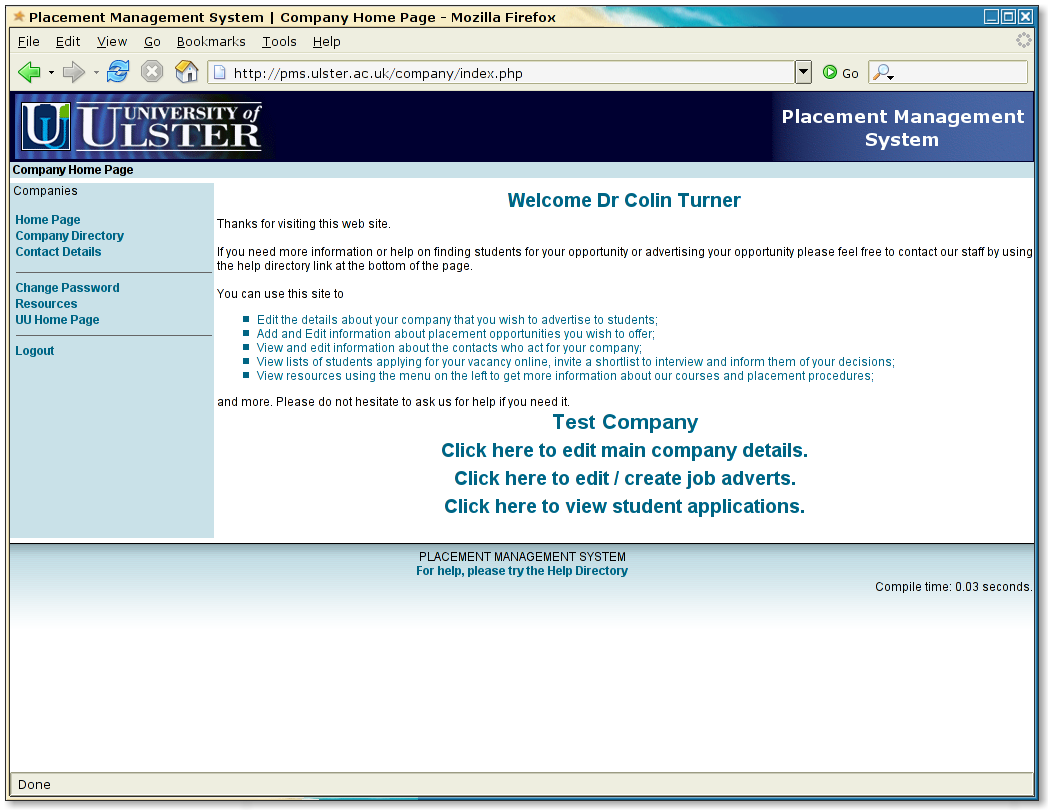
\includegraphics[scale=0.25]{png/company_hr1.png}
\end{center}
\end{figure}
On the left hand side you will see a menu. That menu will remain available to you
at all times. At any time clicking on ``Home Page'' will return you here. The other menu
items in turn are

\begin{description}
\item[Company Directory] allows you to search through other companies on the system;
\item[Contact Details] allows you to check and edit your own contact details;
\item[Change Password] allows you to alter the preconfigured password;
\item[Resources] provides a large collection of documents to guide you;
\item[UU Home Page] takes you the main university home page;
\item[Logout] logs you out from the system.
\end{description}

At any time, clicking on the link for the ``Help Directory'' will
provide you with details on the staff who are most likely to be
able to help with your enquiries.


\subsection{Checking the Company Details}

Possibly the first thing you may want to do (especially if this is your first visit to
the system), is to check over the company information. At the bottom of the main screen
it says ``Click here to edit main company details''.

\begin{figure}[htb]
\begin{center}
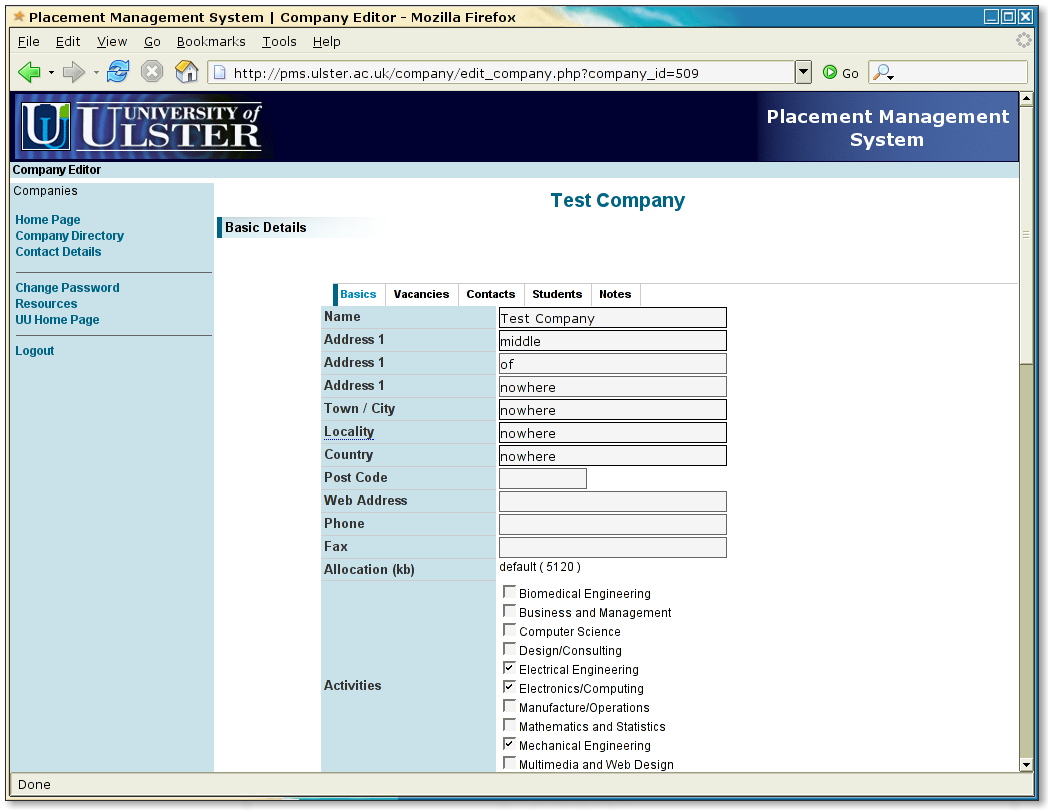
\includegraphics[scale=0.25]{png/company_hr2.png}
\end{center}
\end{figure}


Clicking on this will take you to a page that allows you to edit much about your company,
including the basic contact details. You will also notice that above this area there is
a collection of other headers such as ``Vacancies'' etc., these provide another means of
navigating your record.

Be sure to check your company information is correct. Please note that students are not
shown phone numbers so that they will not bother you directly. You can insert these in the
company brief if you want students to have this information. In the ``Locality'' field please
enter the geographical region of your company. Within the UK and Ireland this could be a
county, or within the areas of larger cities such as Belfast or Dublin please enter the
city name.

Towards the bottom of the form there are other areas to explore.

\begin{figure}[htb]
\begin{center}
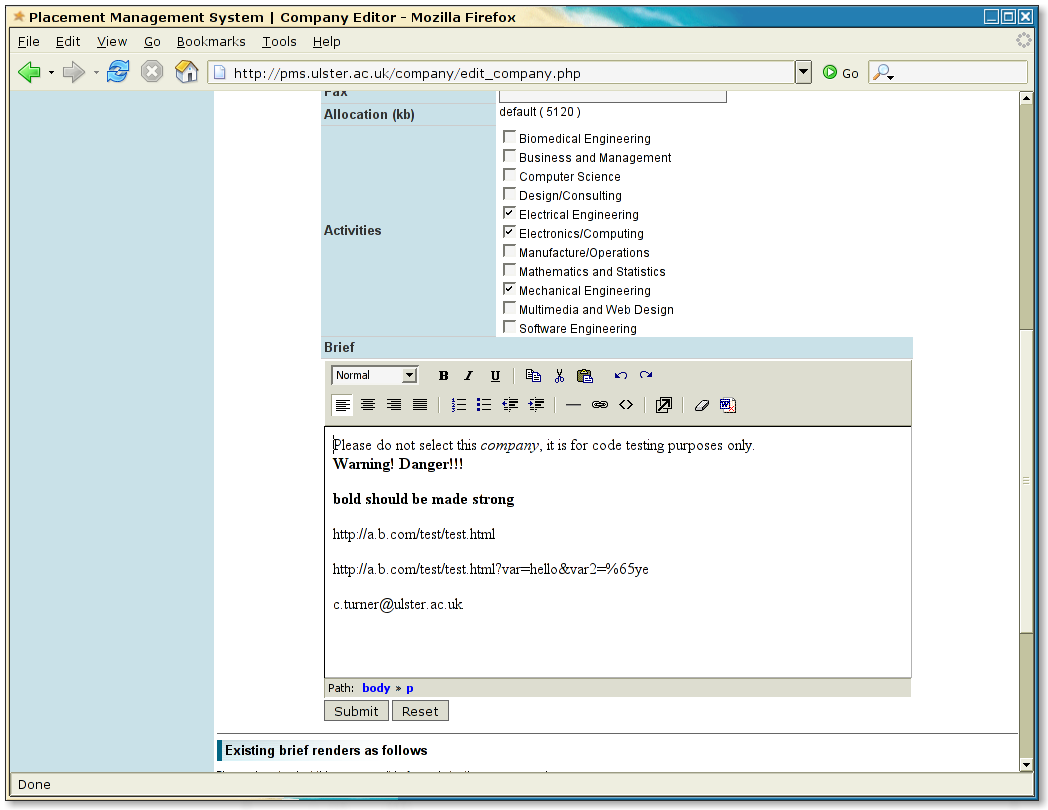
\includegraphics[scale=0.25]{png/company_hr3.png}
\end{center}
\end{figure}


File allocation is an amount of memory for you to use to upload resources, these are PDF
documents to further describe your company, or application forms or similar. If you require more, please contact an administrator
from your help directory.

Activities allows you to indicate in which areas your company does business. Note that you will have a separate opportunity to list activities for your vacancies, so this is a chance to describe all the areas your company is active in.

Finally we have the brief. This is an area in which you can
describe your company to the students. An editor is available in
all modern browsers to allow you to edit this content.

Make your edits as you wish and then save them.

\section{Advertising your vacancy}

Next you will wish to move on to posting your advert for your
vacancy or perhaps you wish to advertise several opportunities.

Clicking on the ``vacancies'' tab of the display will take you
where you need to go
\begin{figure}[htb]
\begin{center}
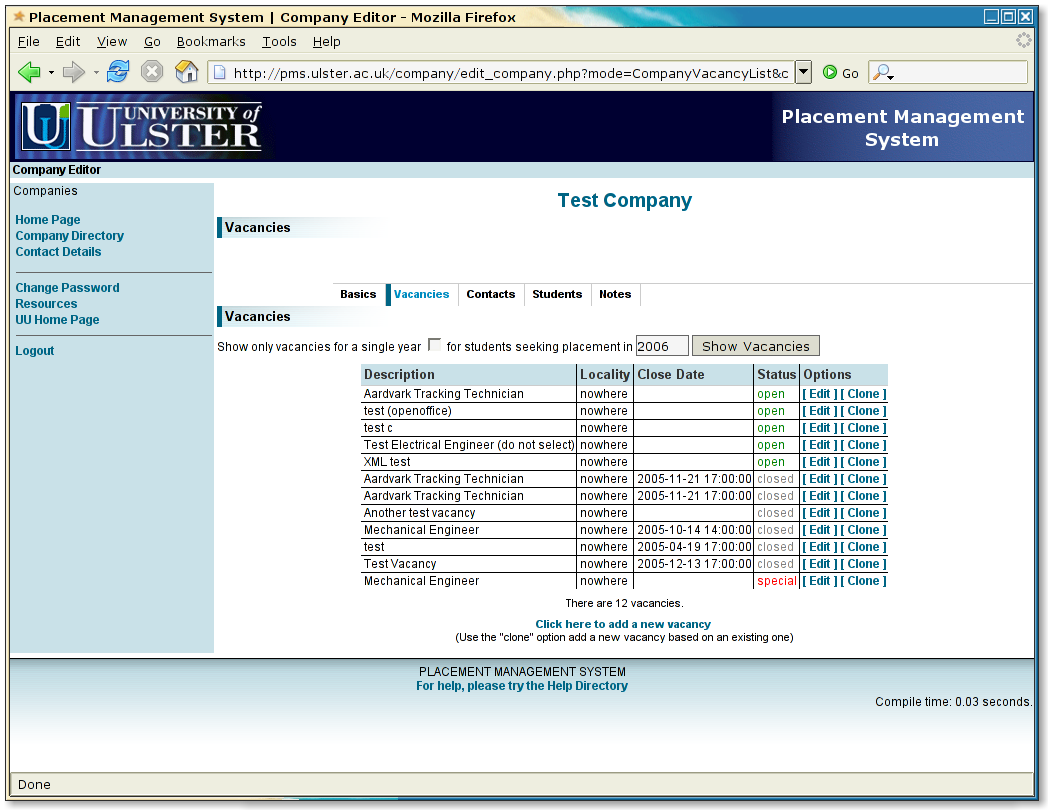
\includegraphics[scale=0.25]{png/company_hr4.png}
\end{center}
\end{figure}


The page will list the vacancies you already have on the system
(if any). You can ``edit'' an existing vacancy, by clicking on
``edit'' to the right. Using the ``clone'' option starts a new
vacancy, but using the existing one as a template to start with.

Many times you will want to create a new vacancy from scratch,
and for this click on the link at the bottom of the page.

Adding a vacancy is similar to editing your company brief.
Here are some points to help your

\begin{description}
\item[Description] is a summary of your proposed vacancy. Where
possible be as descriptive as possible, and try to avoid
``placement student''.
\item[Job Start Date] is essential to the system. It will use it to
decide which students should be shown your vacancy. If you are 
unsure use a provisional date in the area you are planning, you
can always change it later.
\item[Application Close Date] is not compulsory, but if you set
one the system will automatically close your vacancy after this
date and email you a notification.
\item[Application Status] can be one of open, closed and special.
Vacancies that are ``open'' can be applied for on-line and you
will be able to use the full facilities of the system. The
status ``special'' indicates vacancies where the application
cannot be made on our website because of some restriction you
may have. Finally ``closed'' indicated applications are no
longer possible. Vacancies will close automatically after the
closing date passes (if you have declared one).
\end{description}

\section{Checking and selecting students}

By clicking on the ``Students'' tab you will be able to see
the applications made to your vacancies. All vacancies will be
listed for a specific year.
\begin{figure}[htb]
\begin{center}
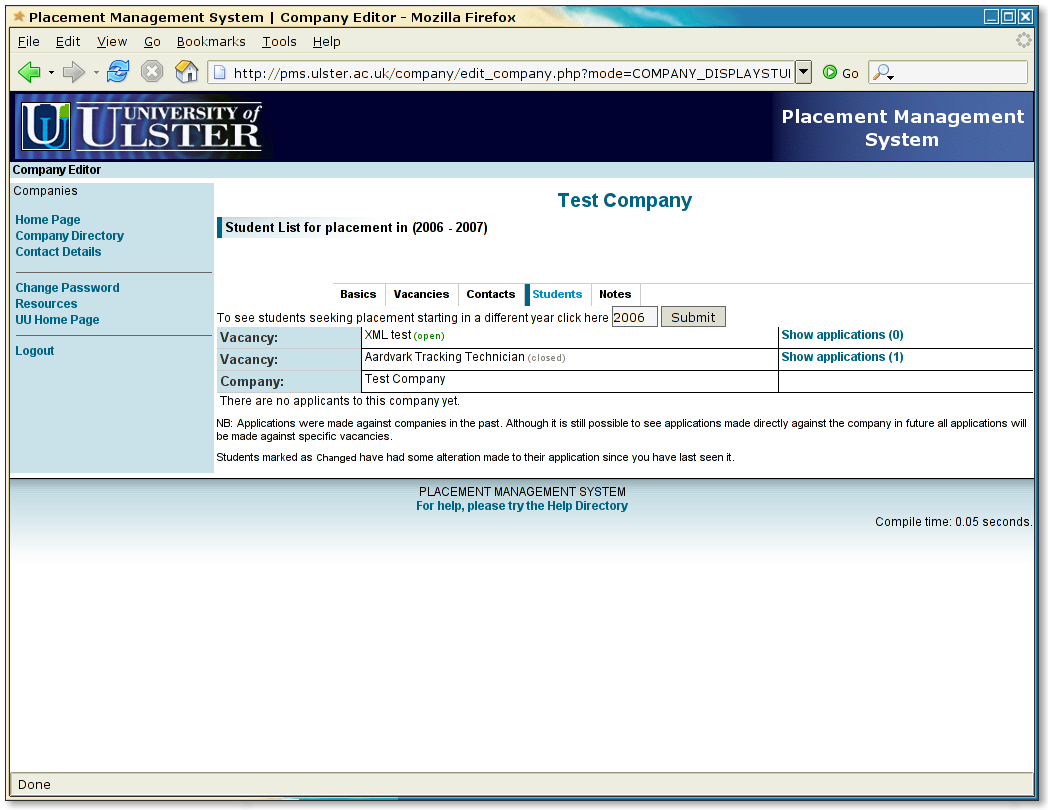
\includegraphics[scale=0.25]{png/company_hr5.png}
\end{center}
\end{figure}

Click on ``Show applications'' for a specific vacancy to see
what students have applied.

Student lists are triaged as follows
\begin{itemize}
\item students you have selected for this vacancy;
\item students who are still available;
\item students who applied but are no longer available (e.g. they are placed elsewhere).
\end{itemize}

For each student you will see
\begin{itemize}
\item their name; clicking on this produces their CV;
\item their course of study;
\item whether their application has changed since you have last seen it;
\item their application date, and any date of modification;
\item a link for who can help with \emph{this} student;
\item a form to allow you to change their status;
\item and a link to request a CV to be emailled to you.
\end{itemize}

You can then call students to email, or use the form to do this
for you.

\section{What Next?}

When you have accepted students you can use the form in their
entry to inform them of this, and we would also ask you to
inform your contact within the university. The university will
then record the student as being placed with your company.


\part{Workplace Supervisor Guide}

\chapter{Using OPUS to help supervise students}

\section{Introduction}

This guide is aimed at helping those people who have day-to-day responsibility
for supervising a placement student from the University of Ulster.

Your student can fill in your details in his or her placement record, using
OPUS at \url{\opusurl}. At that point you will be sent a username and
password to access the system; provided an email address was specified when
your details were added.

This guide explains what this account can be used for, and whether you will want
to use it.

\subsection{Multiple Accounts}

Please note that you may already have a user on OPUS, in which case that account
probably has a different purpose (for example, to be used to recruit students in the
first place). You should continue to keep the credentials for that account in addition
to your supervisor account.

If you supervise several students you may find you receive several accounts for use
in supervising these students. Please retain all the credentials for each account
until the placements are complete.

\section{Getting Started}.

If you have not already got an account on the OPUS then please speak to your normal contact
for placement within the University, or email
% @todo add an email address here
to have an account made for you.

When you have your login details, you can login at \url{\opusurl}.

When you login, you will see something like the following
\begin{figure}[htb]
\begin{center}
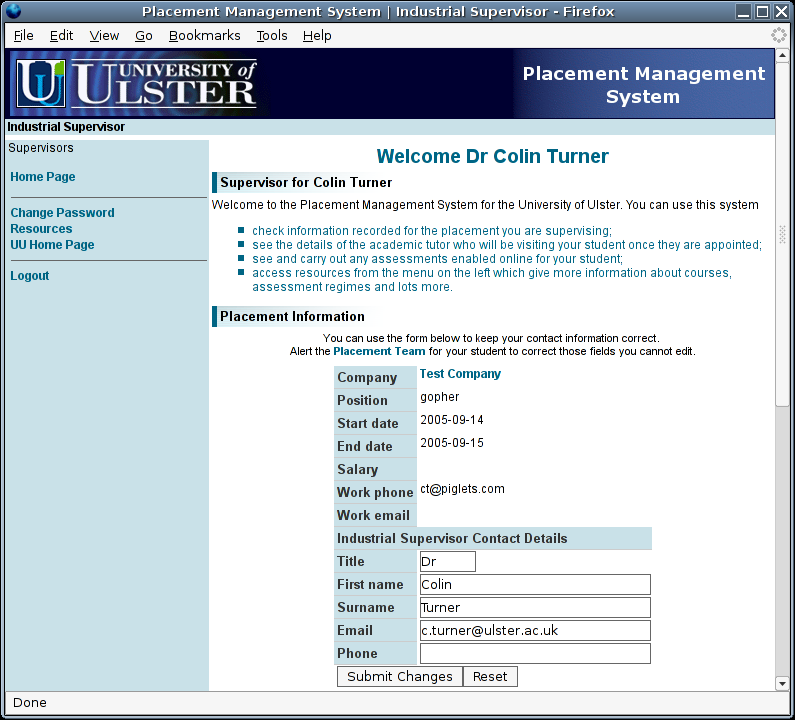
\includegraphics[scale=0.25]{png/supervisor_guide1.png}
\end{center}
\caption{Your home page (top part)}
\end{figure}
On the left hand side you will see a menu. 
At any time clicking on ``Home Page'' will return you here. The other menu
items in turn are

\begin{description}
\item[Change Password] allows you to alter the preconfigured password;
\item[Resources] provides a large collection of documents to guide you;
\item[UU Home Page] takes you the main university home page;
\item[Logout] logs you out from the system.
\end{description}

At any time, clicking on the link for the ``Help Directory'' at the bottom of the page
will provide you with details on the staff who are most likely to be
able to help with your enquiries.

\section{What can you do?}

Here is a summary of what this account offers you.

\subsection{Placement Information}

As you can see, the home page shows some information about the placement. Some of
this cannot be edited for important operational reasons, but you can contact the
staff in the help directory if you need it to be changed.

You will also see your own contact details, which naturally you can edit for your
convenience.

\subsection{Academic Tutor}

Students on placement will also be allocated an academic tutor, although sometimes
this takes some time after the initial placement. If the academic tutor is
appointed you will see their details on-screen.

\begin{figure}[htb]
\begin{center}
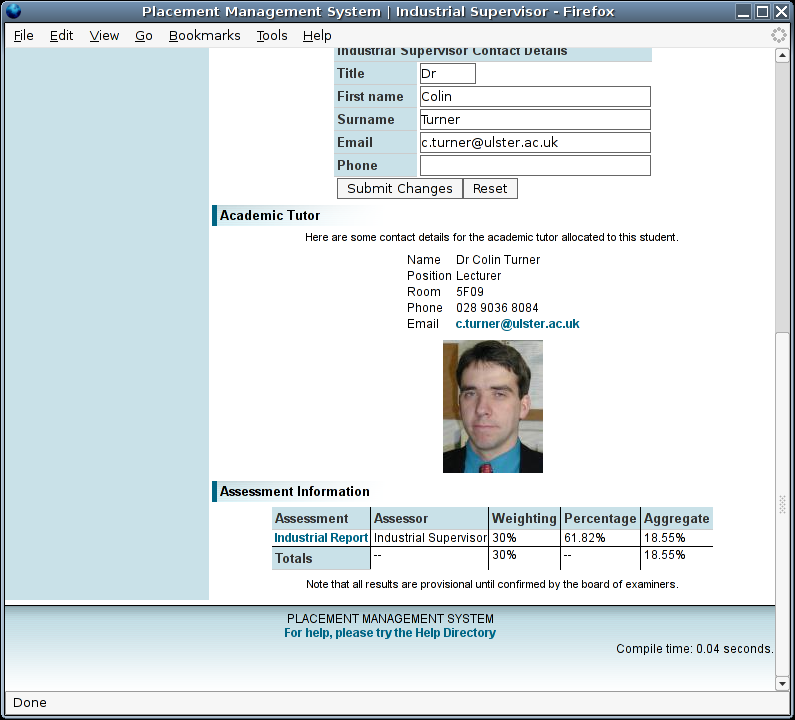
\includegraphics[scale=0.25]{png/supervisor_guide2.png}
\end{center}
\caption{Your home page (bottom part)}
\end{figure}

Usually this staff member will visit the student during the placement, and in any case
provides another important contact if you have any worries or concerns.

\subsection{Assessment}

You may also be invited to file assessments for the student on-line, and if so, the
assessments will be shown on the screen. Simply click on the assessment name to fill
in the assessment at the appropriate time.

\subsection{Help Directory}

Click on the help directory at the bottom of the screen to find out who is available
to help you with any queries you may have about the placement.

\subsection{Resources}

When you click on \emph{resources} on the left, you will be shown a list of documents
that may help you managing this placement.


\part{Student Guide}

%
%
%

\chapter{OPUS and PDP}

\section{PDP}

\section{The PDSystem}

%
%
%

\chapter{Preparing for and Getting a Placement}

\section{CVs}

\section{Covering Letters}

\section{e-Portfolios}

\section{Searching for vacancies}

\section{Applying for vacancies}

\section{Managing applications}

\section{Health \& Safety}

\section{Self assessments}

%
%
%


\chapter{Using OPUS while on placement}

\section{Announcements}

\section{Resources}

\section{Assessment}

%
%
%

\chapter{OPUS after your placement}

\section{Assessment}

\section{Learning the lessons}

%
% Index
%

\printindex
\markboth{Index}{}
\addcontentsline{toc}{chapter}{Index}

\end{document}



